\section{Employment Dynamics}
The next question we can ask is how health types differ when it comes to employment status and earnings. Is health type a good predictor for labour market participation? Are there clear correlations between health types and sociodemographic features such as sex, education, and earnings?

The answer seems to be affirmative. Both Type~II and Type~III reflect higher unemployment rates than the UKHLS sample average; Type~II is more than double the sample's 4.1\% unemployment rate at 8.63\%. It is important to note that the ``inactive'' category includes students, those who are sick or disabled, individuals engaged in family care, and various types of retirees. Given that the cohort spans ages 38--70, such classification matters for interpretation.

To further elucidate the relationship between health types and labour market outcomes, I examine employment rates and average earnings by cluster and age. This analysis is particularly relevant in the context of increasing retirement ages across developed countries, driven by fiscal deficits \citep{bbc2023_pension}. While my primary focus is on health types, retirement policy context informs the interpretation of differential labour market attachment \citep{usnews_retirement}.

\begin{itemize}
    \item \textbf{Employment rates.} Types~II and III (frail health groups) show lower employment rates both before and after the typical retirement age of 60--67 \citep{usnews_retirement}.
    \item \textbf{Average hourly earnings.} Type~I: \pounds13.11 (above sample average); sample average: \pounds12.95; Type~II: \pounds8.86 (31.6\% below average); Type~III: \pounds9.84 (24.0\% below average).
\end{itemize}

These disparities in earnings are striking, with Types~II and III earning approximately 25\% less than the sample average. While post-retirement individuals in the sample may influence these figures, the distinct characteristics of the three health types persist across age groups. This analysis underscores the profound impact of health trajectories on both employment prospects and earning potential.

\begin{table}[ht]
    \centering
    \caption{Average hourly earnings and unemployment rates by health type}
    \label{tab:earnings}
    \begin{tabular}{lrr}
        \toprule
        Group & Avg. Hourly Earnings (\pounds) & Unemployment Rate (\%) \\
        \midrule
        Sample average & 12.95 & 4.10 \\
        Type I & 13.11 & --- \\
        Type II & 8.86 & 8.63 \\
        Type III & 9.84 & --- \\
        \bottomrule
    \end{tabular}
    \begin{flushleft}
    \footnotesize Note: ``---'' indicates the rate was not explicitly reported in the text.
    \end{flushleft}
\end{table}


Education differences reinforce these labour market gaps:
\begin{itemize}
    \item \textbf{University degree attainment.} Type~I: 42.7\%; Type~II: 27.3\%; Type~III: 23.1\%.
    \item \textbf{A-level attainment.} Consistent across all types at approximately 20--23\%.
\end{itemize}

The most striking feature is the markedly higher proportion of degree-holders in Type~I compared to Types~II and III. This sharp contrast suggests a strong association between higher education and more favorable health trajectories. The consistency in A-level attainment across all types indicates that the main educational divergence occurs in the progression to university rather than in secondary school achievement.

These findings underscore the complex interplay between education, health, and socioeconomic status. They highlight the need for further investigation into the causal relationships between educational attainment and health outcomes, as well as potential interventions to address educational disparities that may contribute to divergent health trajectories.

\begin{table}[ht]
    \centering
    \caption{Educational attainment by health type}
    \label{tab:education}
    \begin{tabular}{lrr}
        \toprule
        Health Type & University Degree (\%) & A-level Attainment (\%) \\
        \midrule
        Type I & 42.7 & 20--23 \\
        Type II & 27.3 & 20--23 \\
        Type III & 23.1 & 20--23 \\
        \bottomrule
    \end{tabular}
\end{table}


\begin{figure}[ht]
    \centering
    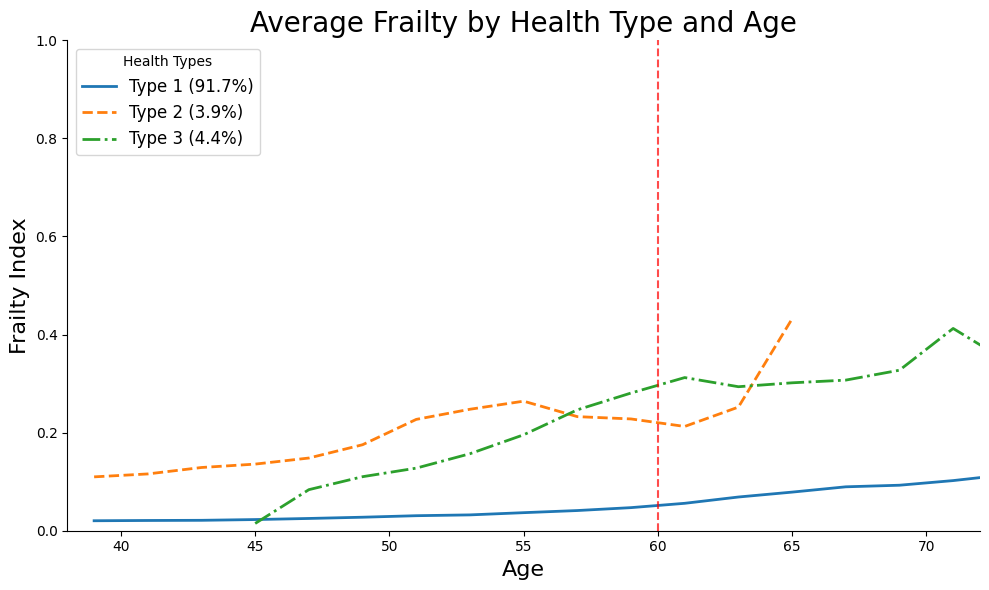
\includegraphics[width=0.85\textwidth]{figures/fig-010.png}
    \caption{Labour market outcomes by health type (extracted from the original dissertation PDF).}
    \label{fig:employment}
\end{figure}
